\documentclass[aspectratio=169]{beamer}
\usepackage[utf8]{inputenc}
\usepackage[spanish]{babel}
\usepackage{graphicx}
\usepackage{amsmath}
\usepackage{amsfonts}

% --- CONFIGURACIÓN DE COLORES INSTITUCIONALES USS ---
\definecolor{USSBlue}{RGB}{0, 32, 91}    % Azul marino
\definecolor{USSGold}{RGB}{212, 175, 55} % Dorado

\mode<presentation> {
  \usetheme{Madrid}
  \usecolortheme[named=USSBlue]{structure}
  \setbeamercolor{palette primary}{bg=USSBlue,fg=white}
  \setbeamercolor{palette secondary}{bg=USSBlue,fg=white}
  \setbeamercolor{palette tertiary}{bg=USSBlue,fg=white}
  \setbeamercolor{title}{bg=white,fg=USSBlue}
  \setbeamercolor{item}{fg=USSGold}
  \setbeamertemplate{navigation symbols}{} 
}

% --- DATOS DE PORTADA ---
\title[Robótica Industrial]{Modelamiento Cinemático de un Brazo Robótico 2D}
\subtitle{Taller de Aptitudes Lógicas y Matemáticas}
\author[M. Amundarain, F. Ramírez, J.P Vargas]{Moisés Amundarain, Fernando Ramírez, Juan Pablo Vargas}
\institute[USS]{
  Ingeniería Civil Informática \\
  Facultad de Ingeniería \\
  \textbf{Universidad San Sebastián}
}
\date{13 de Mayo, 2026}

% --- COMENTARIO: Logo de la Universidad ---
\titlegraphic{
\includegraphics[width=6cm]{logo_uss.png}}

\begin{document}

% 1. PORTADA
\begin{frame}
  \titlepage
\end{frame}

% 2. DEFINICIÓN DEL PROBLEMA: SUPUESTOS
\begin{frame}{Definición del Problema: Supuestos}
  \begin{columns}
    \begin{column}{0.5\textwidth}
      \textbf{Contexto Operacional:}
      \begin{itemize}
        \item \textbf{Movimiento Planar:} El brazo opera estrictamente en un plano cartesiano bidimensional (ejes X e Y).
        \item \textbf{Rigidez:} Los eslabones se consideran elementos indeformables.
        \item \textbf{Precisión:} Se busca determinar la posición exacta de la herramienta mediante giros angulares.
      \end{itemize}
    \end{column}
    \begin{column}{0.5\textwidth}
      \begin{center}
        % COMENTARIO: Insertar imagen 1 aquí
        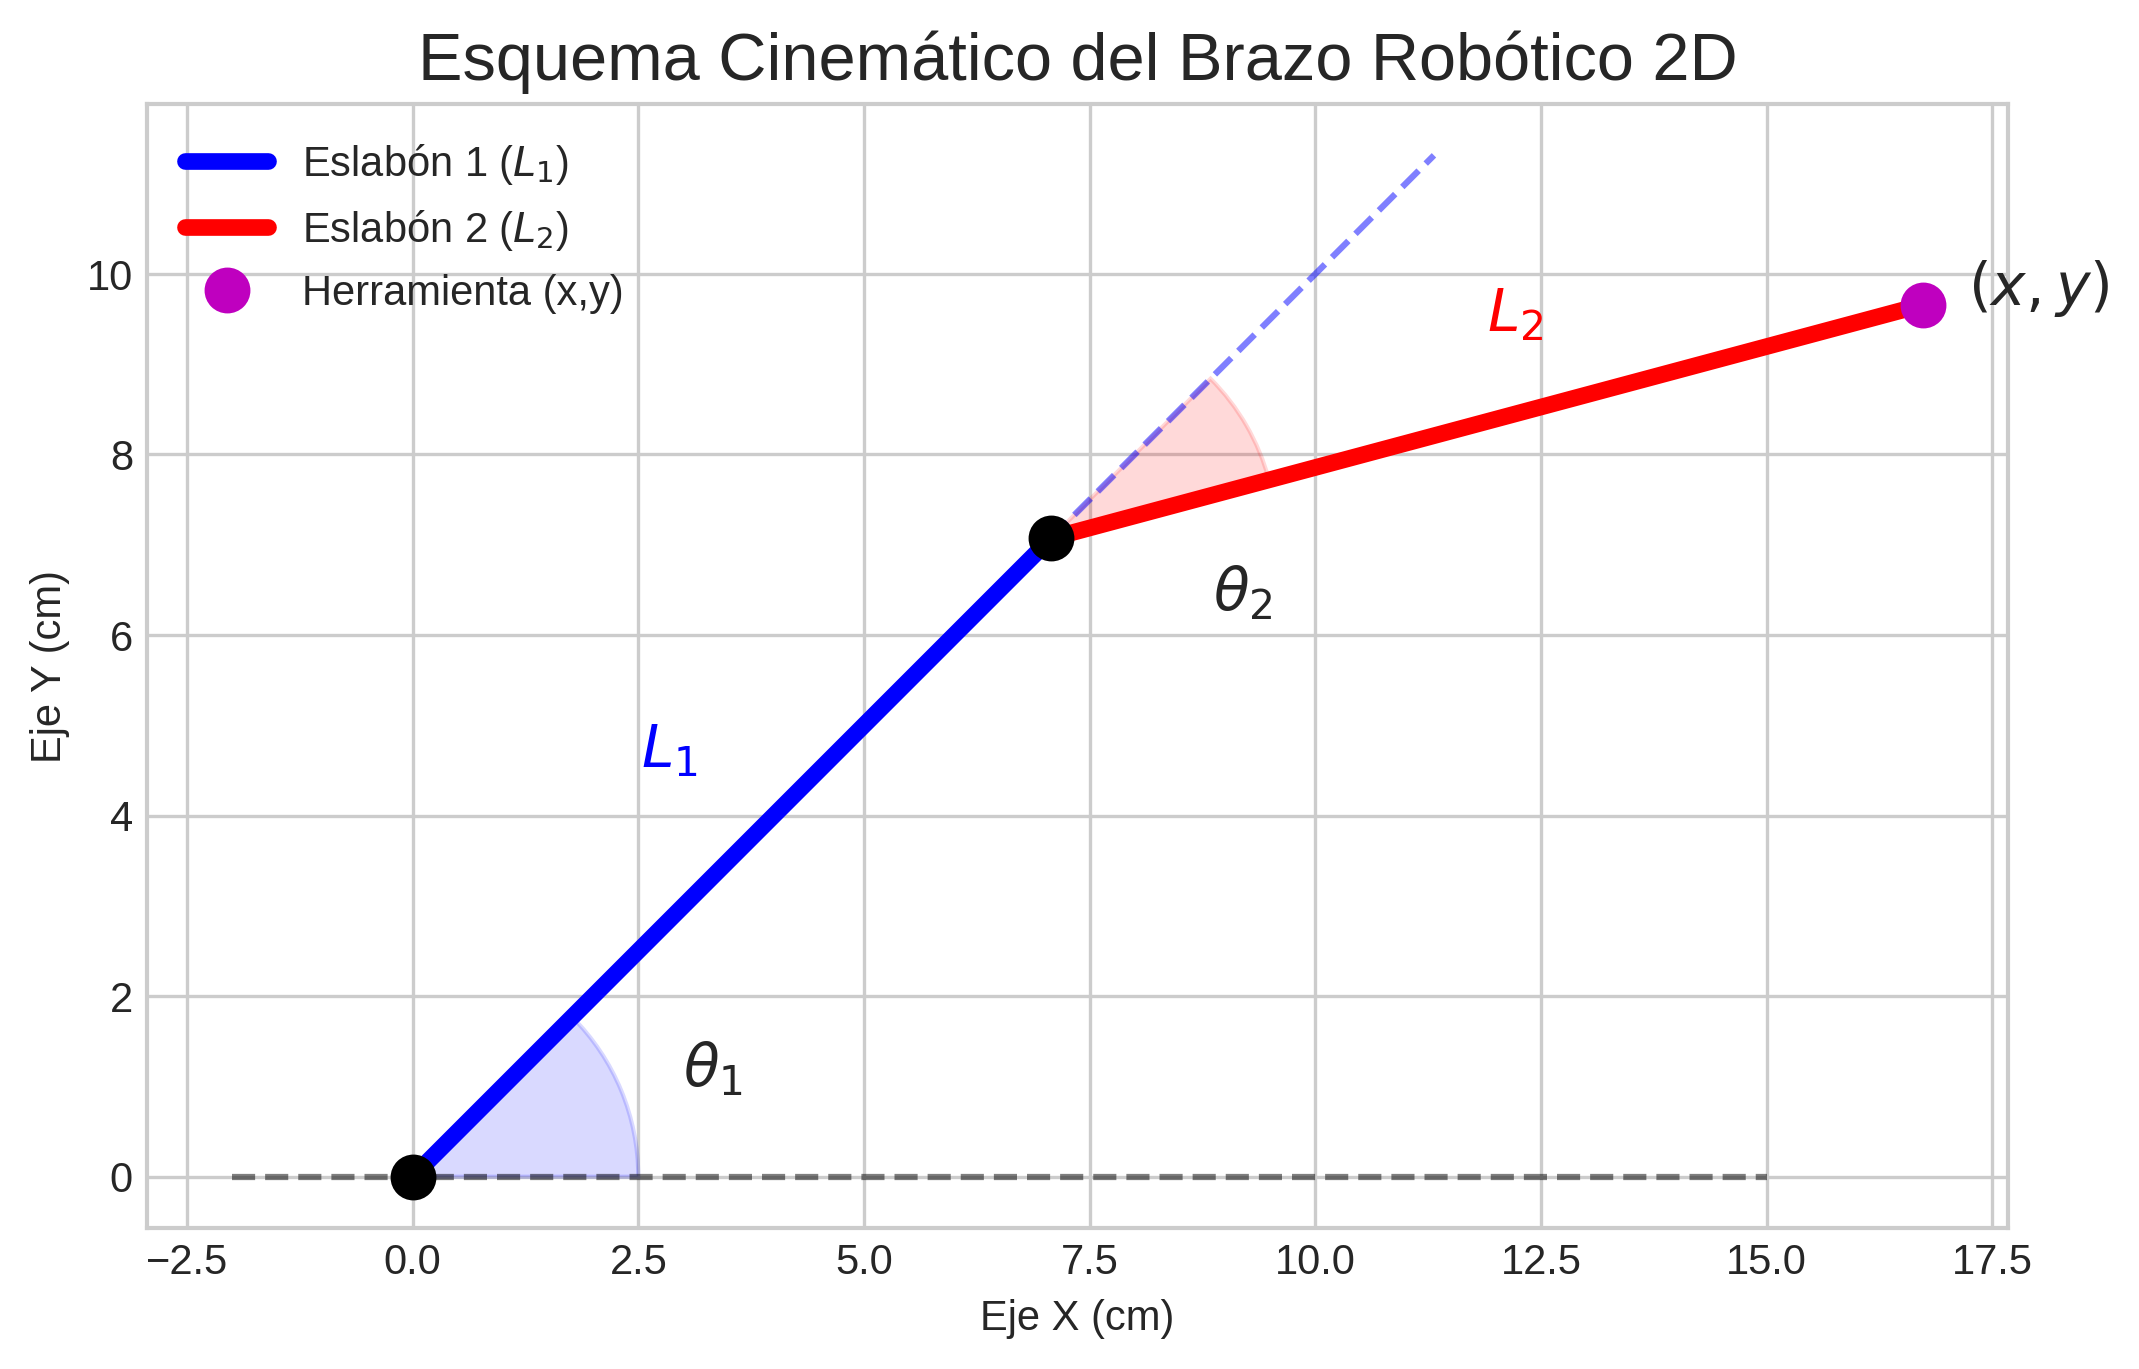
\includegraphics[width=0.95\textwidth]{1_esquema_brazo.png}
      \end{center}
    \end{column}
  \end{columns}
\end{frame}

% 3. DEFINICIÓN DEL PROBLEMA: VARIABLES
\begin{frame}{Definición del Problema: Variables}
  \begin{columns}
    \begin{column}{0.5\textwidth}
      \textbf{Parámetros y Variables:}
      \begin{itemize}
        \item \textbf{Longitudes (Constantes):} \\ $L_1 = 10$ cm, $L_2 = 10$ cm.
        \item \textbf{Entradas (Independientes):} \\ Ángulos $\theta_1$ (base) y $\theta_2$ (codo).
        \item \textbf{Salidas (Dependientes):} \\ Coordenadas cartesianas $(x, y)$.
      \end{itemize}
    \end{column}
    \begin{column}{0.5\textwidth}
      \begin{center}
        % COMENTARIO: Insertar imagen 1 aquí (Muestra variables)
        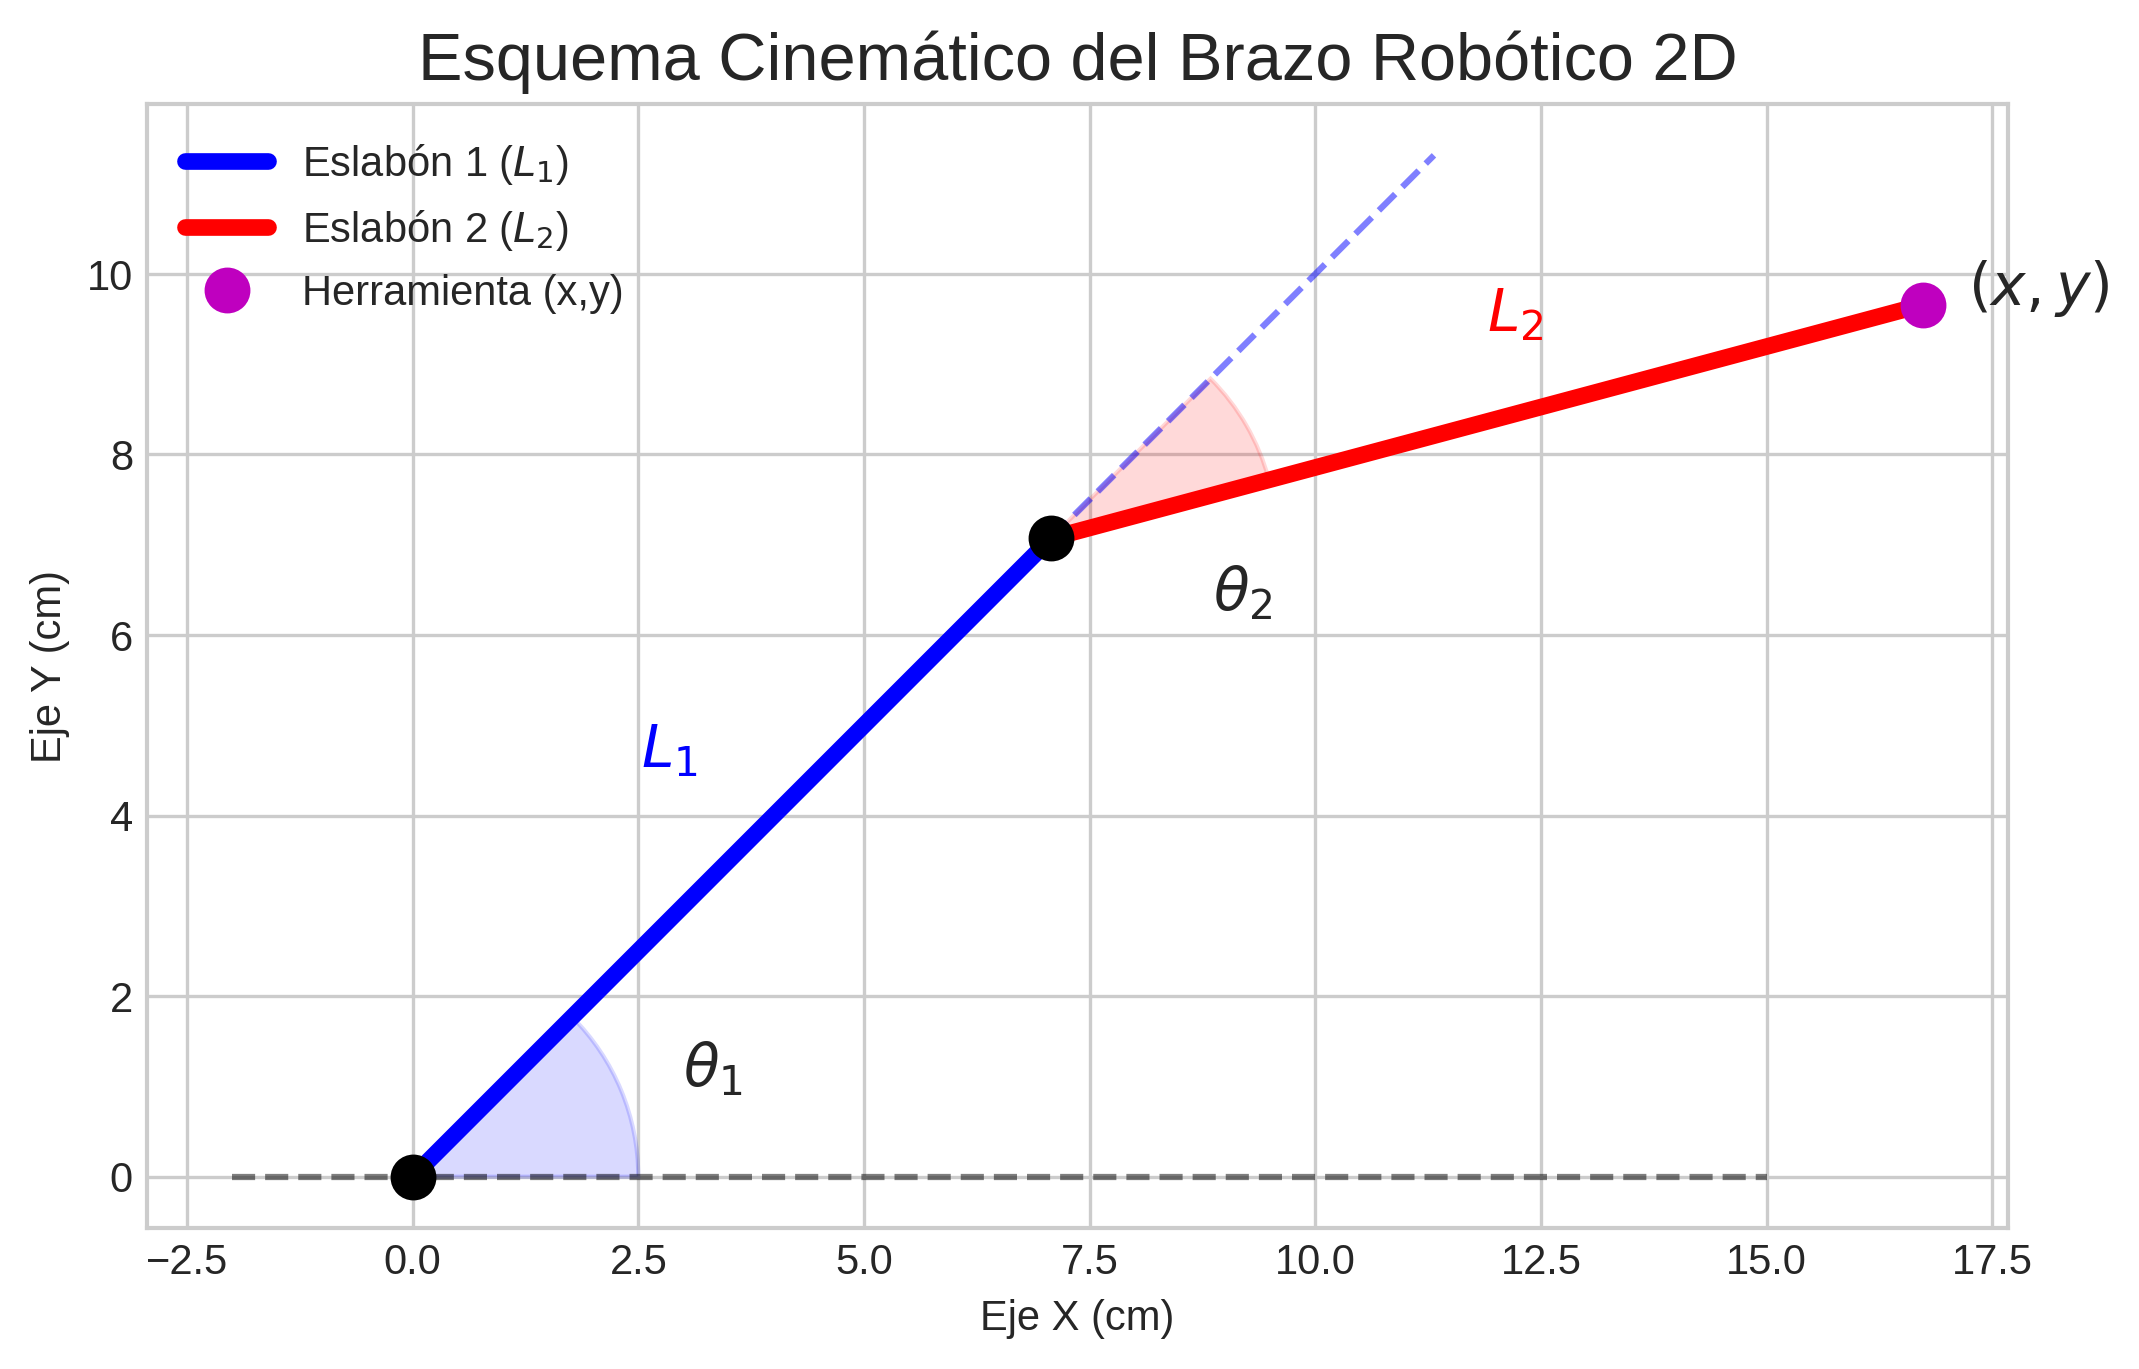
\includegraphics[width=0.95\textwidth]{1_esquema_brazo.png}
      \end{center}
    \end{column}
  \end{columns}
\end{frame}

% 4. MODELAMIENTO: JUSTIFICACIÓN
\begin{frame}{Modelamiento: Justificación Algebraica}
  \begin{columns}
    \begin{column}{0.5\textwidth}
      \textbf{¿Por qué Trigonometría?}
      \begin{itemize}
        \item Permite descomponer vectores de posición en sus componentes ortogonales.
        \item Relaciona el carácter dinámico del giro con una posición estática.
        \item \textbf{Coseno:} Proyección sobre el eje X.
        \item \textbf{Seno:} Proyección sobre el eje Y.
      \end{itemize}
    \end{column}
    \begin{column}{0.5\textwidth}
      \begin{center}
        % COMENTARIO: Insertar imagen 2 aquí
        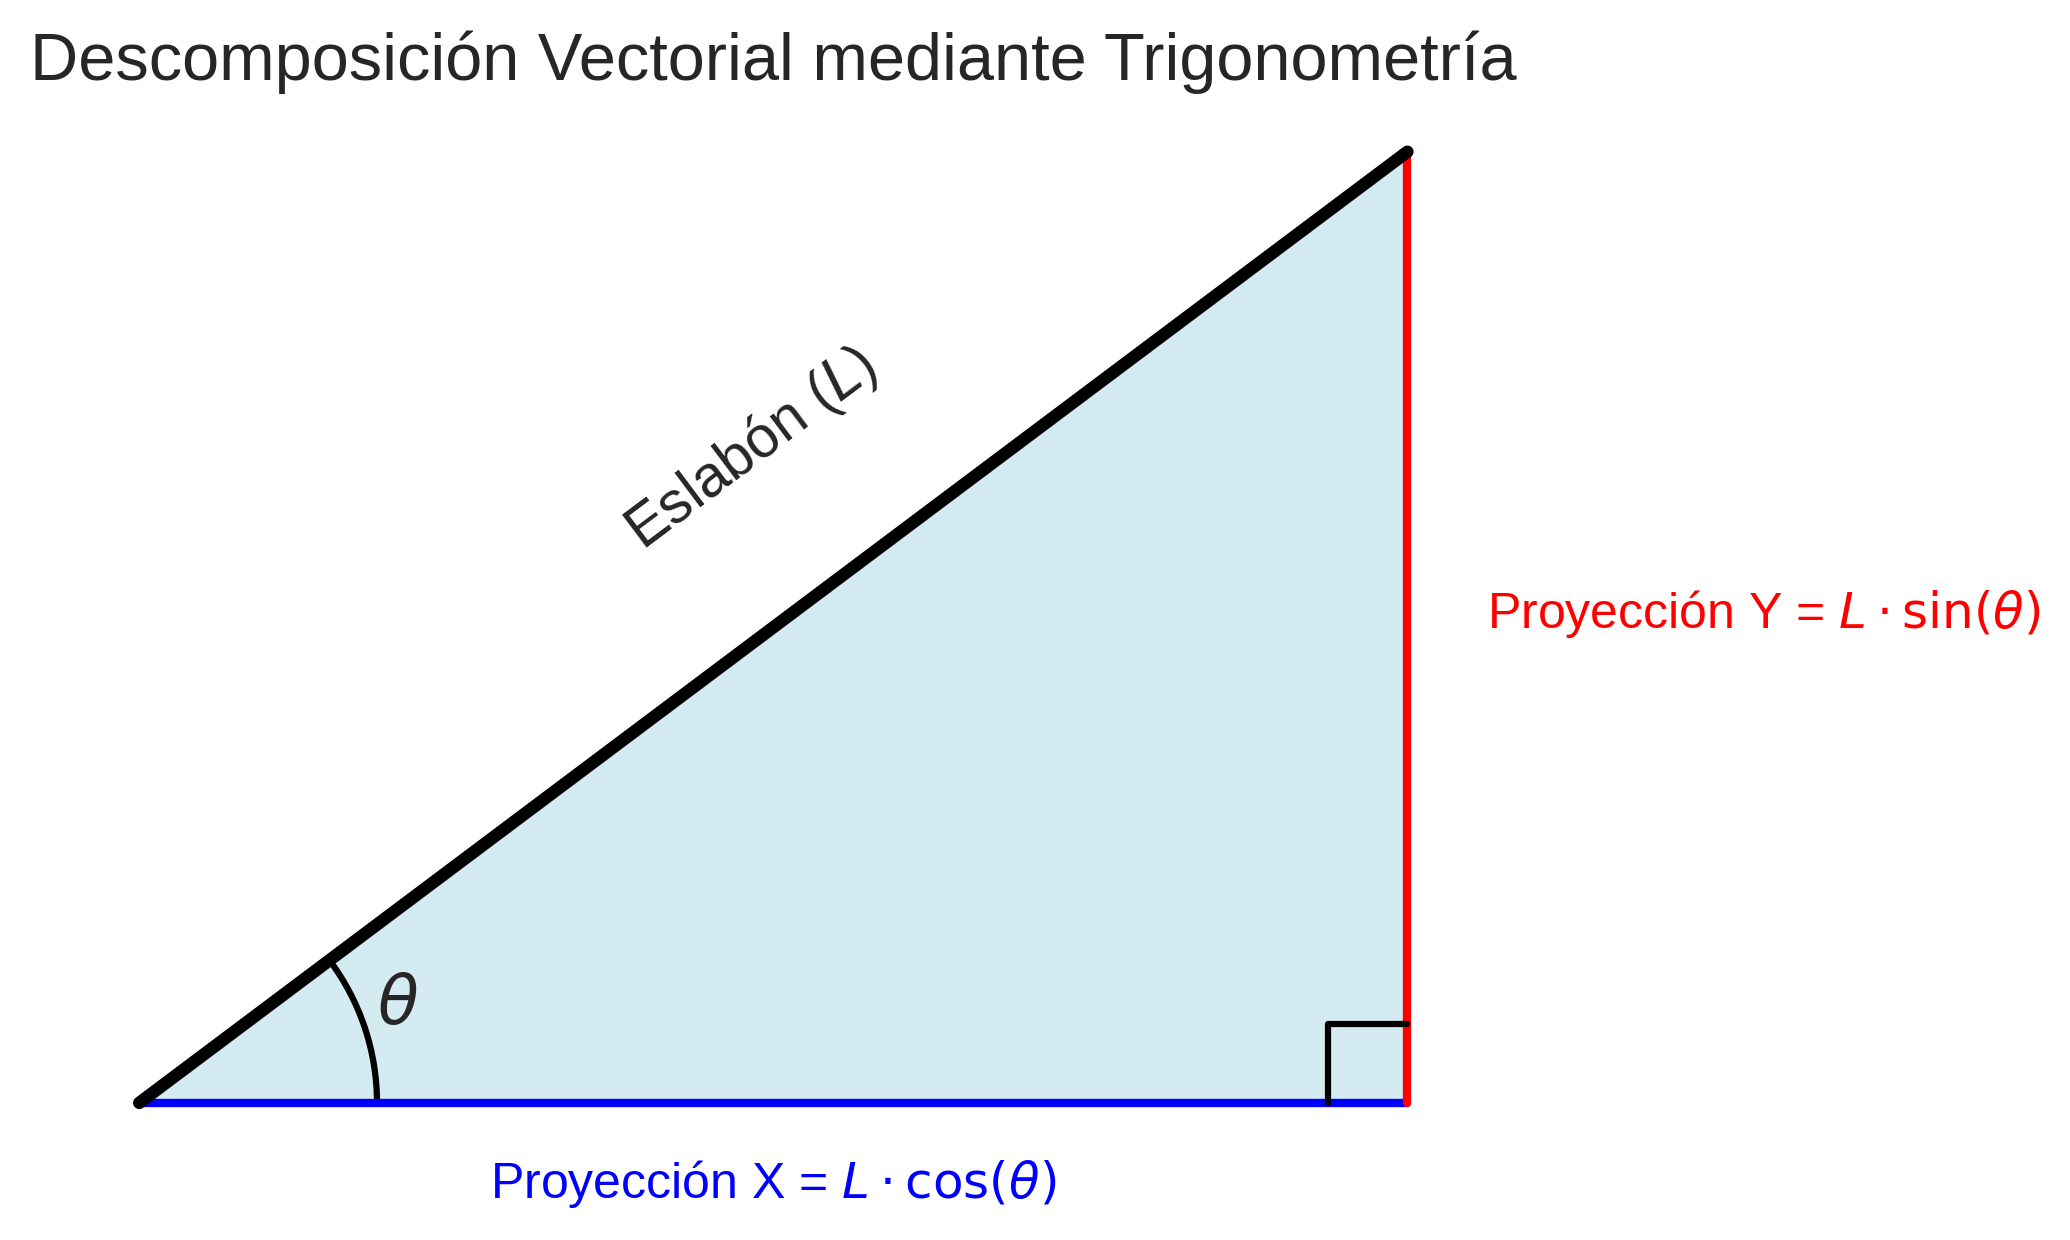
\includegraphics[width=0.9\textwidth]{2_triangulo_trigo.png}
      \end{center}
    \end{column}
  \end{columns}
\end{frame}

% 5. MODELAMIENTO: ECUACIONES
\begin{frame}{Modelo Matemático: Cinemática Directa}
  \begin{block}{Ecuaciones del Sistema}
    Para determinar la posición $(x, y)$ de la herramienta, sumamos las proyecciones de ambos eslabones:
    \begin{align*}
      x &= L_1 \cos(\theta_1) + L_2 \cos(\theta_1 + \theta_2) \\
      y &= L_1 \sin(\theta_1) + L_2 \sin(\theta_1 + \theta_2)
    \end{align*}
  \end{block}
  \vspace{0.4cm}
  \centering
  \textit{Este modelo permite coordinar los motores para alcanzar puntos específicos en el plano.}
\end{frame}

% 6. VALIDACIÓN: PUNTO A
\begin{frame}{Validación: Punto A (Reposo)}
  \begin{columns}
    \begin{column}{0.5\textwidth}
      \textbf{Configuración Inicial:} \\
      $\theta_1 = 0^\circ, \theta_2 = 0^\circ$
      
      \vspace{0.3cm}
      \textbf{Cálculo Manual:}
      \begin{itemize}
        \item $x = 10\cos(0) + 10\cos(0) = 20$ cm.
        \item $y = 10\sin(0) + 10\sin(0) = 0$ cm.
      \end{itemize}
      \vspace{0.3cm}
      \textbf{Resultado:} Coordenada $(20, 0)$. El brazo está totalmente extendido.
    \end{column}
    \begin{column}{0.5\textwidth}
      \begin{center}
        % COMENTARIO: Insertar imagen 3 aquí (Punto A)
        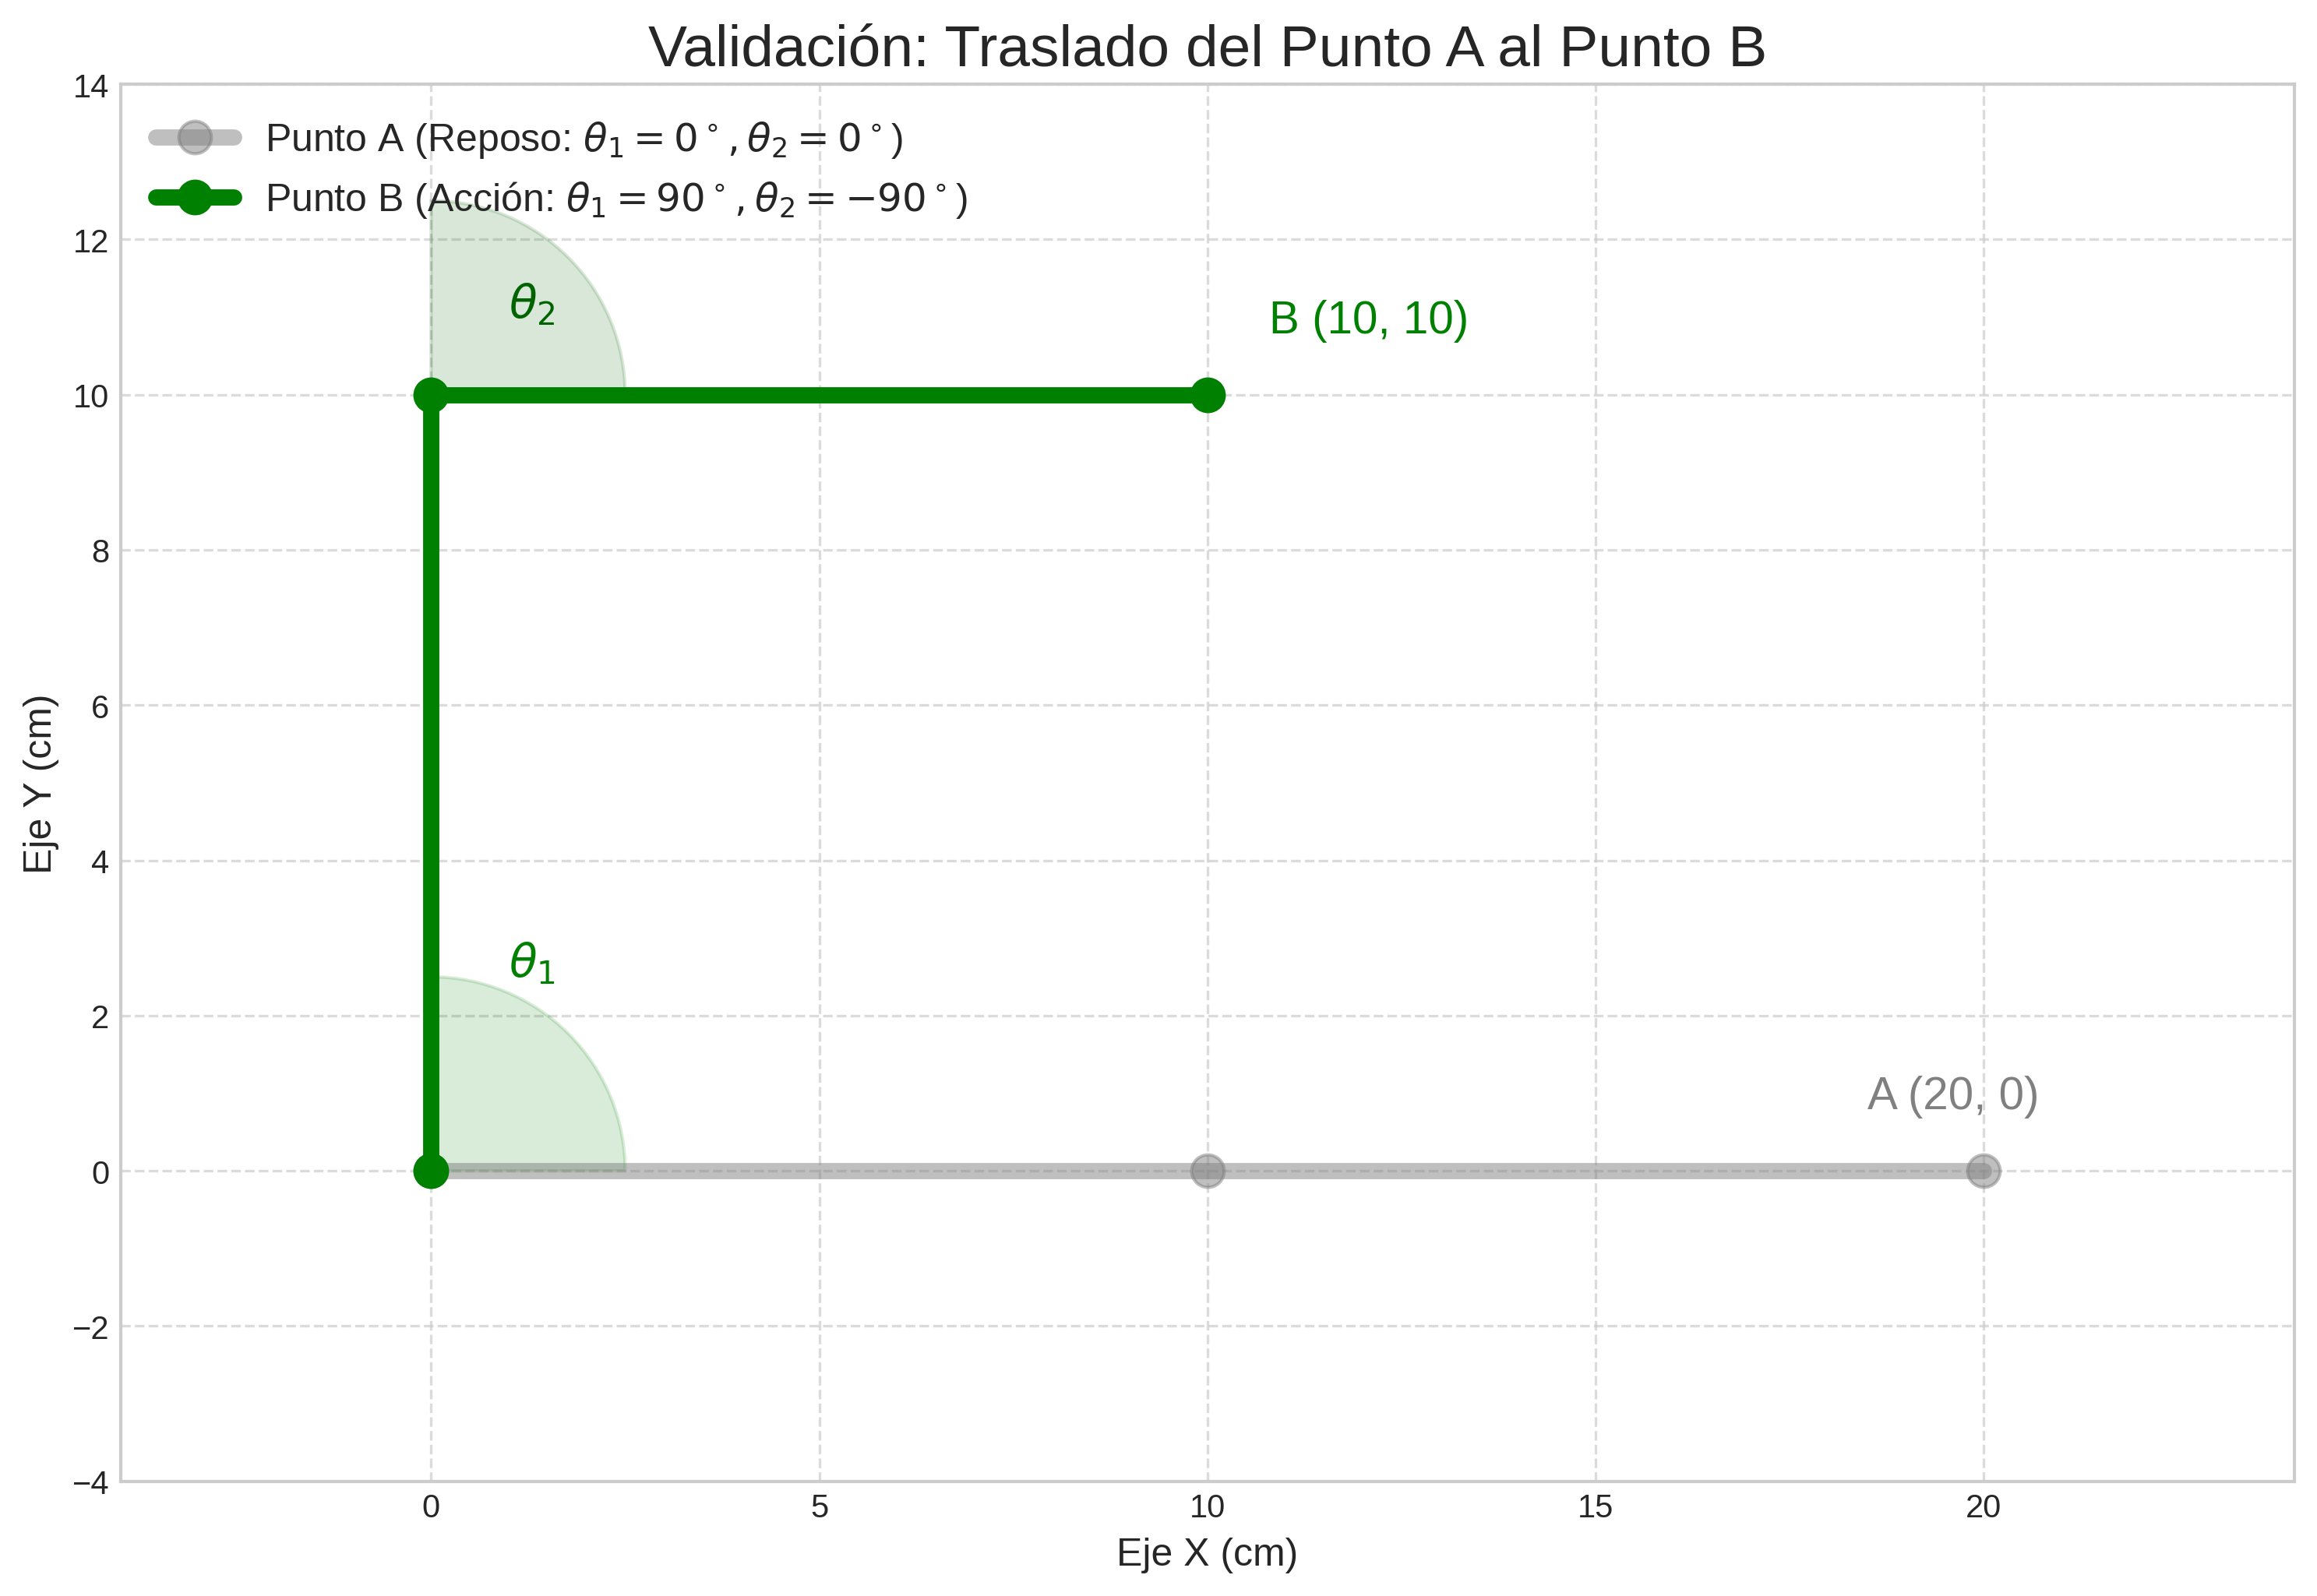
\includegraphics[width=0.9\textwidth]{3_validacion_puntos.png}
      \end{center}
    \end{column}
  \end{columns}
\end{frame}

% 7. VALIDACIÓN: PUNTO B
\begin{frame}{Validación: Punto B (Acción)}
  \begin{columns}
    \begin{column}{0.5\textwidth}
      \textbf{Configuración de Trabajo:} \\
      $\theta_1 = 90^\circ, \theta_2 = -90^\circ$
      
      \vspace{0.3cm}
      \textbf{Cálculo Manual:}
      \begin{itemize}
        \item $x = 10\cos(90) + 10\cos(0) = 10$ cm.
        \item $y = 10\sin(90) + 10\sin(0) = 10$ cm.
      \end{itemize}
      \vspace{0.3cm}
      \textbf{Resultado:} Coordenada $(10, 10)$. El brazo se posiciona para recoger una pieza.
    \end{column}
    \begin{column}{0.5\textwidth}
      \begin{center}
        % COMENTARIO: Insertar imagen 3 aquí (Punto B)
        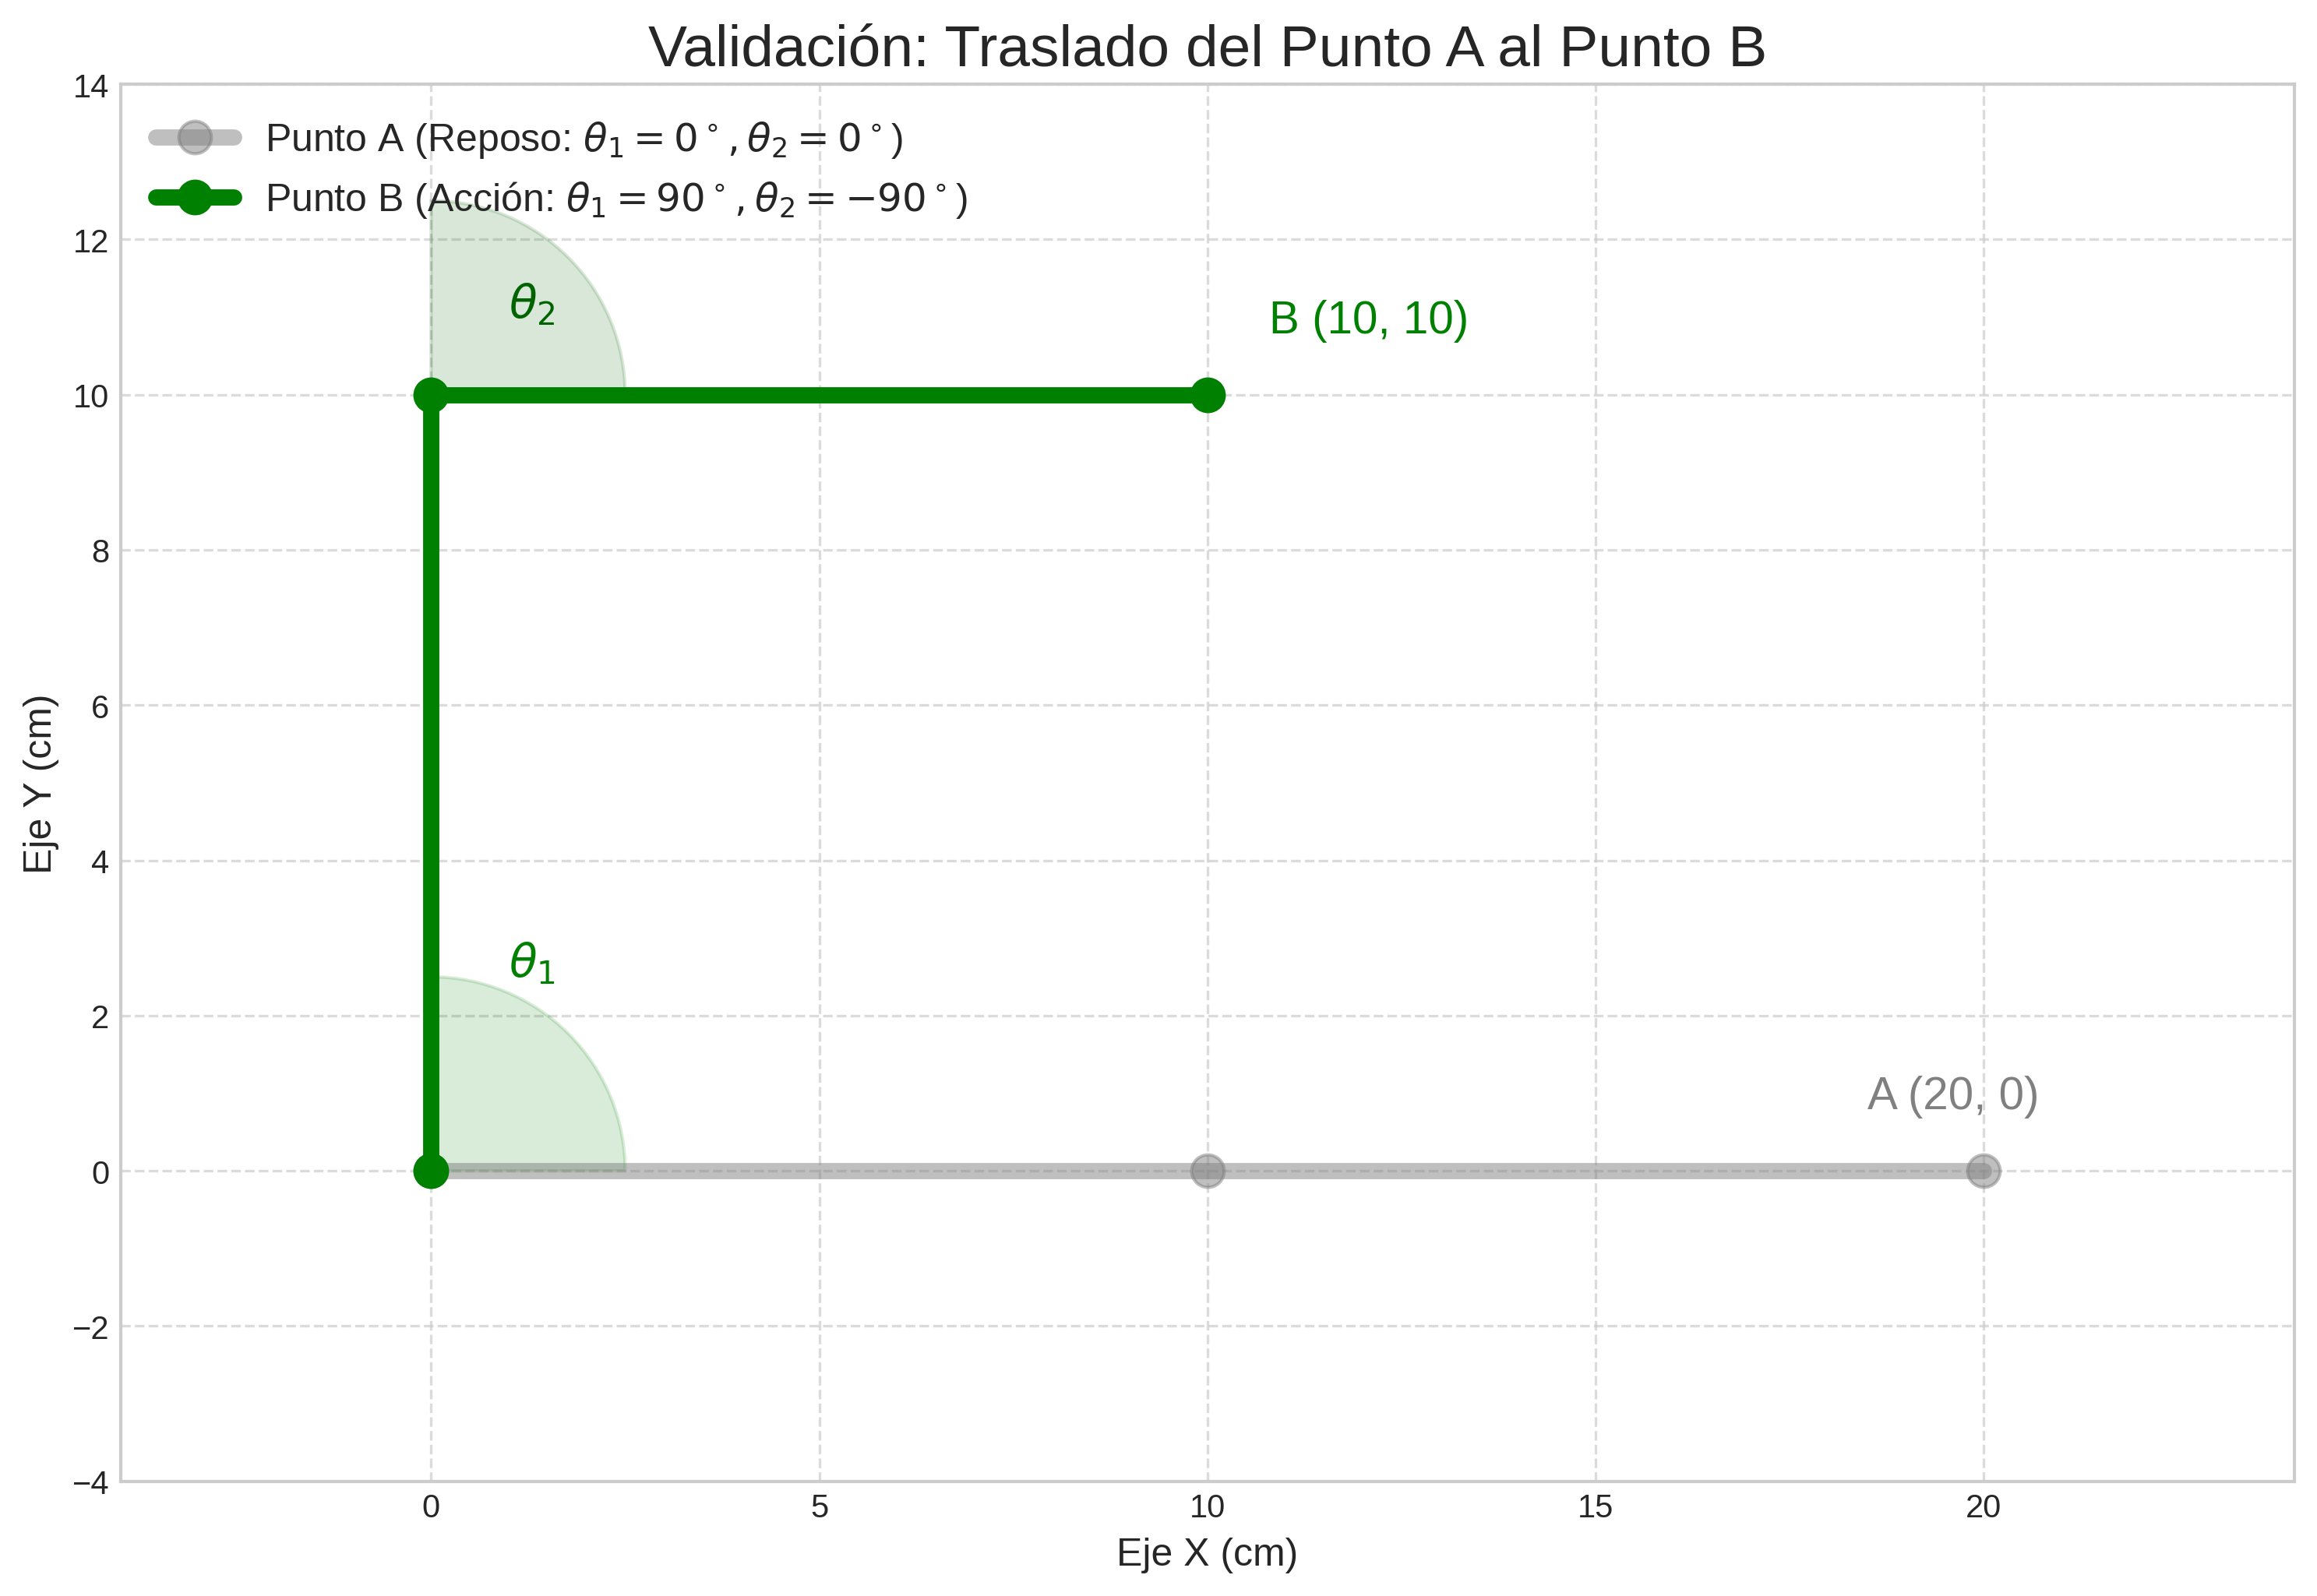
\includegraphics[width=0.9\textwidth]{3_validacion_puntos.png}
      \end{center}
    \end{column}
  \end{columns}
\end{frame}

% 8. RAZONAMIENTO Y LÍMITES
\begin{frame}{Análisis de Límites Físicos}
  \begin{columns}
    \begin{column}{0.5\textwidth}
      \textbf{Razonabilidad de Magnitud:}
      \begin{itemize}
        \item El alcance máximo es $L_1 + L_2 = 20$ cm.
        \item Puntos fuera de este radio son \textbf{inalcanzables}.
        \item Esto demuestra la coherencia del modelo trigonométrico con la realidad física del robot.
      \end{itemize}
    \end{column}
    \begin{column}{0.5\textwidth}
      \begin{center}
        % COMENTARIO: Insertar imagen 4 aquí
        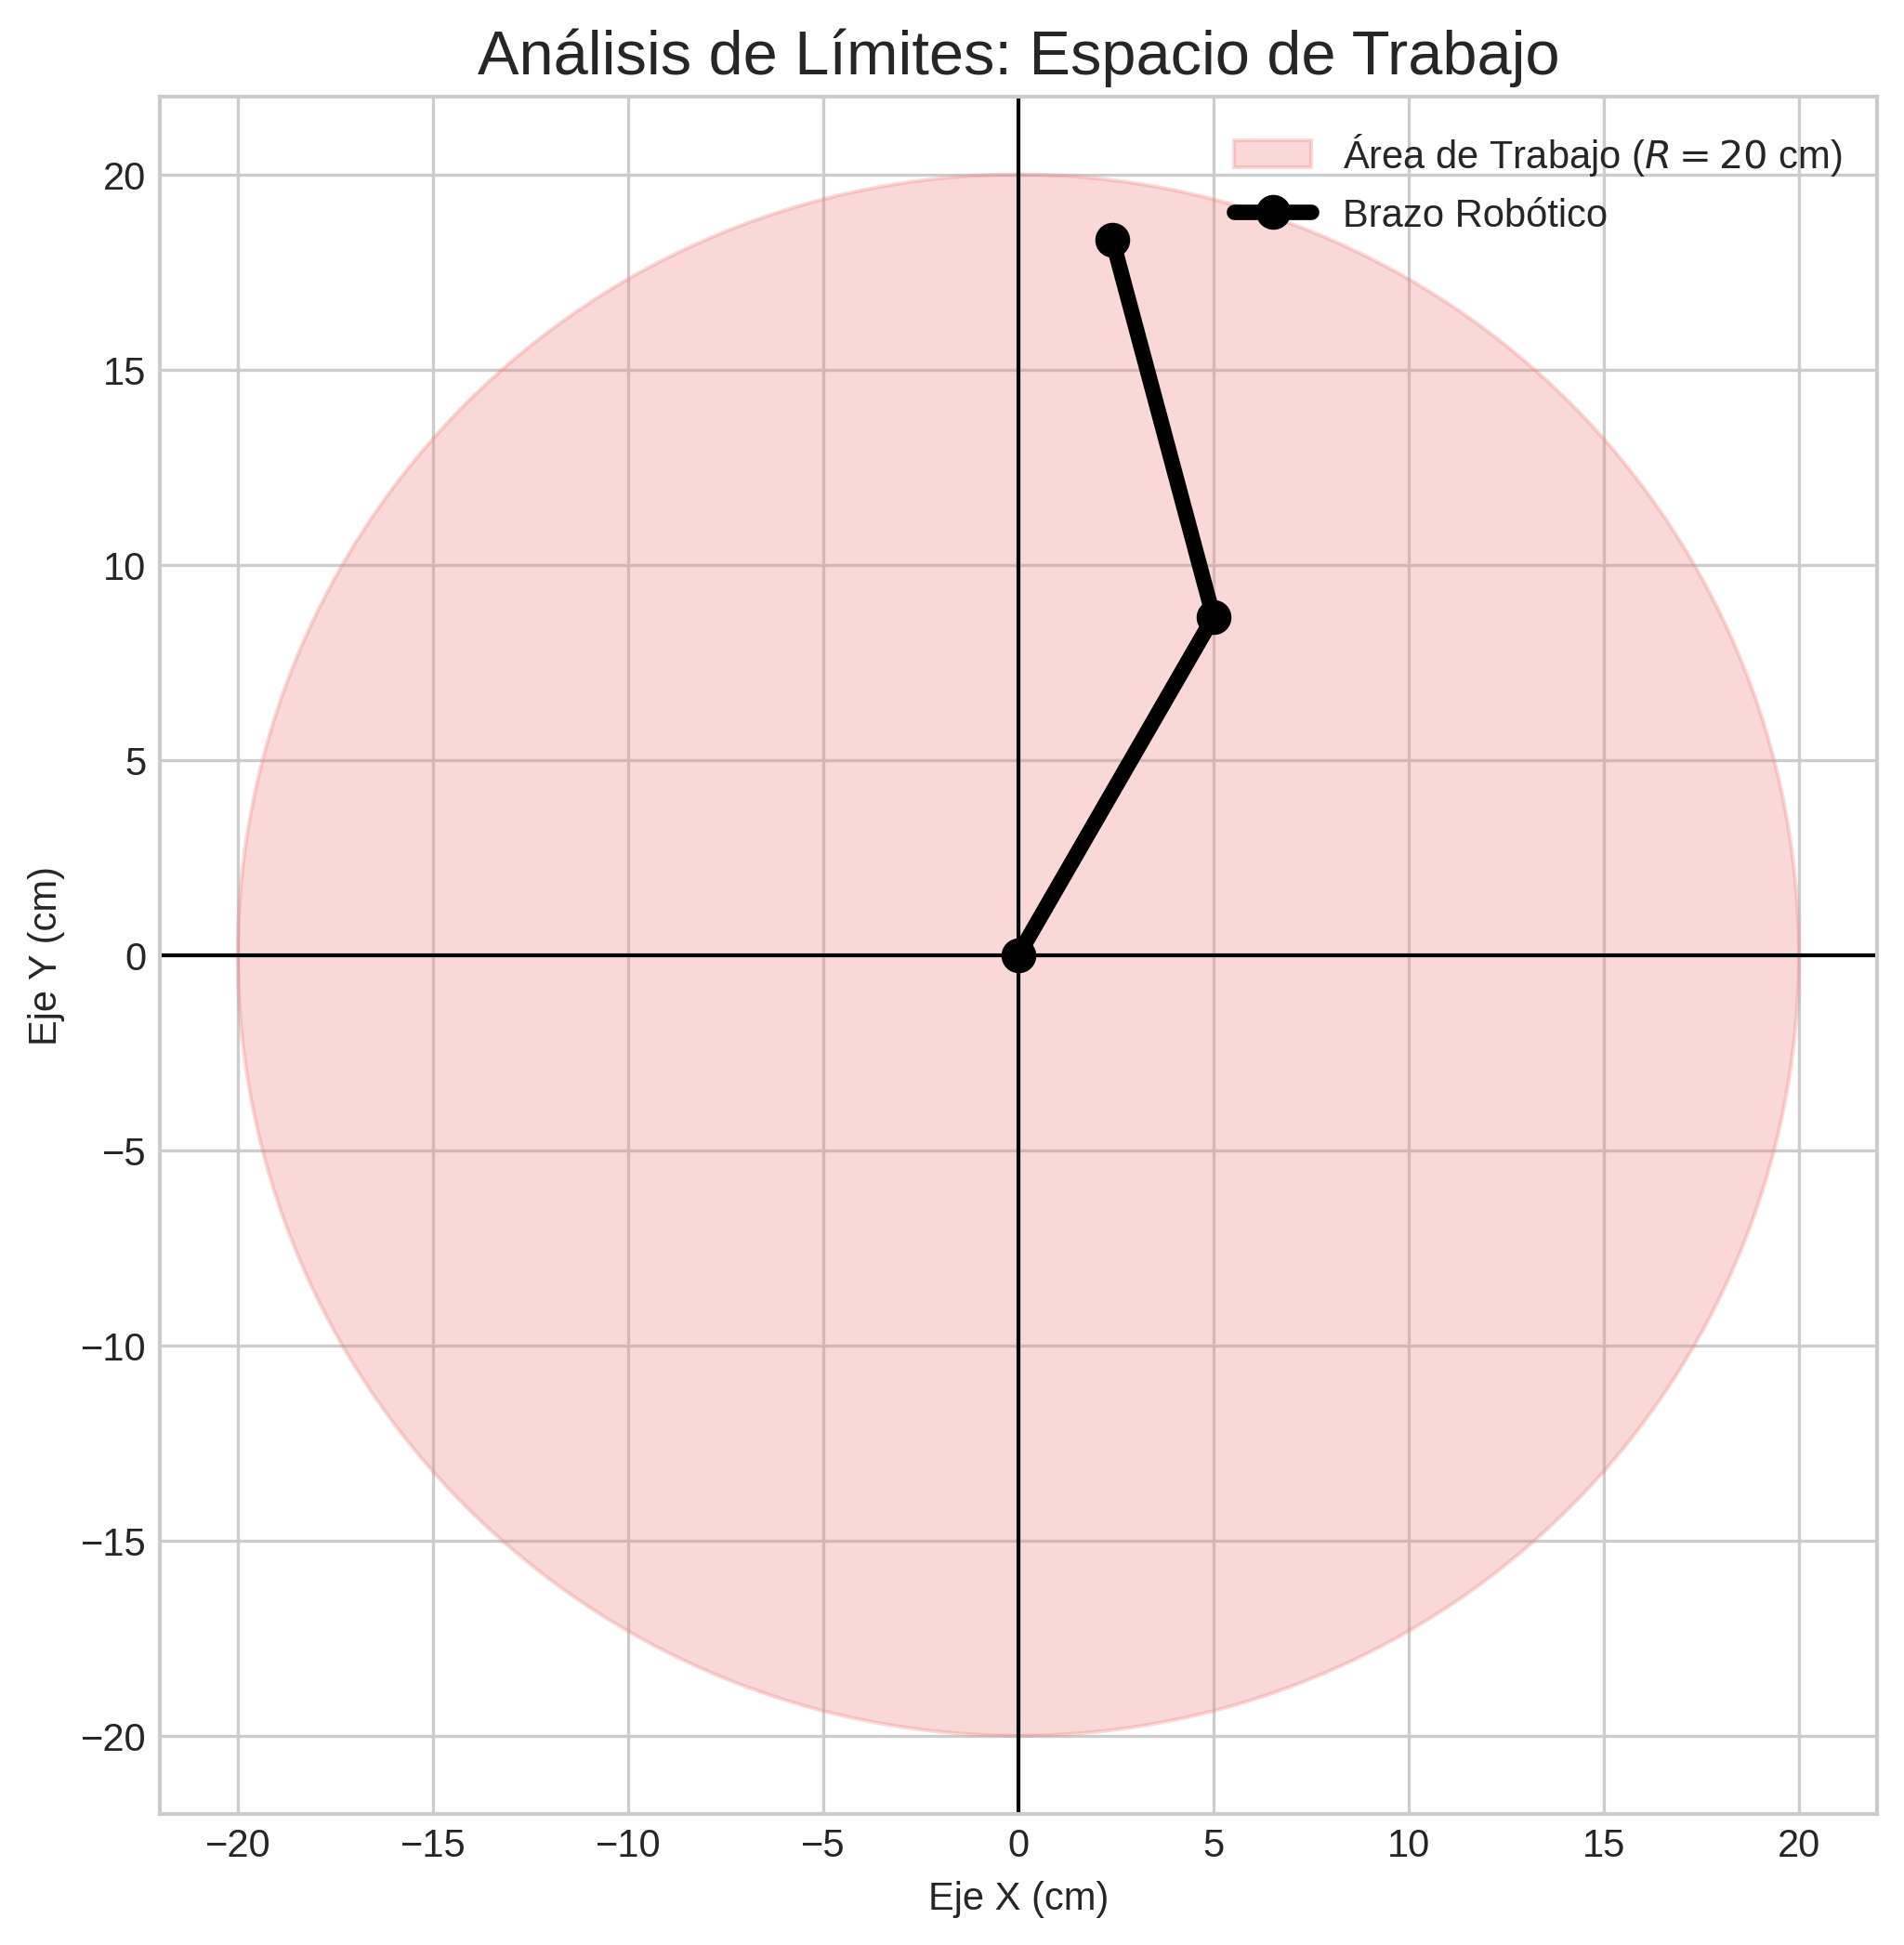
\includegraphics[width=0.95\textwidth]{4_area_trabajo.png}
      \end{center}
    \end{column}
  \end{columns}
\end{frame}

% 9. CONCLUSIÓN
\begin{frame}{Conclusión}
  \begin{itemize}
    \item \textbf{Efectividad:} Se logró vincular variables angulares dinámicas con una posición exacta en el plano mediante proyecciones algebraicas.
    \item \textbf{Validación:} La comprobación manual coincide plenamente con los resultados gráficos de Python, asegurando la fiabilidad del modelo.
    \item \textbf{Seguridad:} El análisis de límites permite definir un área de trabajo segura, fundamental en entornos industriales.
    \item \textbf{Síntesis:} La matemática descriptiva es la herramienta base para la programación de sistemas autónomos complejos.
  \end{itemize}
\end{frame}

\begin{frame}
	\begin{center}
		
\includegraphics[width=8cm]{logo_uss.png}
	\end{center}
\end{frame}

\end{document}